\documentclass[hyperref,xcolor=table]{beamer}
\usepackage{beamerthemesplit}
\usepackage{graphicx}
\usepackage{mathptmx}           % replacement for obsolete \usepackage{times}
\usepackage[scaled=1.0]{helvet} % replacement for obsolete \usepackage{times}
\usepackage{courier}            % replacement for obsolete \usepackage{times}
\usepackage[normalem]{ulem}



\usepackage{tikz}
\usepackage{../tikz-dependency,pifont}
\usetikzlibrary{shapes.arrows,chains,positioning,automata,trees,calc}
\usetikzlibrary{patterns,matrix}
\usetikzlibrary{decorations.pathmorphing,decorations.markings}
\usepackage{times,latexsym,amsfonts,amssymb,amsmath,graphicx,url,bbm,rotating,siunitx}
\usepackage{multirow,hhline,arydshln,array,stmaryrd,pifont,color,centernot}
\usepackage[absolute,overlay]{textpos}
\definecolor{darkred}{rgb}{0.5, 0.0, 0.0}
\definecolor{darkgreen}{rgb}{0.0, 0.4, 0.0}
\definecolor{darkblue}{rgb}{0.0, 0.0, 0.5}
\definecolor{orange}{rgb}{0.767, 0.450, 0.0}
\definecolor{verylightgray}{rgb}{0.9, 0.9, 0.9}

% set up Beamer style with Stanford colors and logo
% logo is available at http://nlp.stanford.edu/local/nlp-logos/nlp-logo.pdf
\useinnertheme{rounded}
\useoutertheme{infolines}
\usecolortheme{beaver}
\setbeamercolor{block title}{fg=white,bg=darkred!75!black}
\setbeamercolor{block body}{parent=normal text,bg=black!5!bg}
\setbeamercolor{item projected}{bg=darkred}
\setbeamertemplate{enumerate items}[default]
\logo{
\includegraphics[height=1cm]{../img/nlp-logo.pdf}}
\renewcommand{\footnoterule}{}
\renewcommand*{\thefootnote}{\fnsymbol{footnote}}

% title page information
\title[Learning Knowledge From Text]{Learning Open Domain Knowledge from Text}
\subtitle{}
\author{Gabor Angeli}
\date{November 5, 2015}
\institute[Stanford]{Stanford University}

\input ../macros.tex
\input ../figures_naturalli.tex
\input ../figures_kbp.tex


\def\roadmap#1{
\begin{frame}[t,noframenumbering]{Roadmap}
\vspace{-0.5ex}
\begin{tabular}{m{3cm} m{7.75cm}}
  
  \ifnum0#1=1
    \rowcolor{verylightgray}
  \fi
  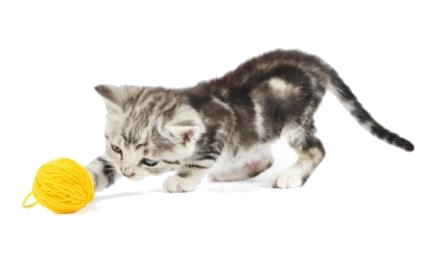
\includegraphics[width=3cm]{../img/yarn-cat.png}
  &
  \hh{Common Sense Reasoning:} \newline \w{Cats have tails} \newline \footnotesize{\cite{key:2013angeli-truth,key:2014angeli-naturalli}} \\
  \\
  
  \ifnum0#1=2
    \rowcolor{verylightgray}
  \fi
  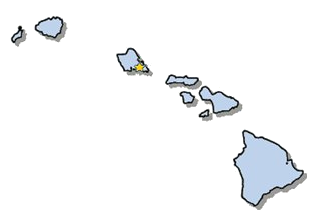
\includegraphics[width=3cm]{../img/hawaii.png}
  &
  \hh{Complex premises:} \newline \w{Born in Hawaii, Obama is a graduate of Columbia} \newline \footnotesize{\cite{key:2015angeli-openie}} \\
  \\

  \ifnum0#1=3
    \rowcolor{verylightgray}
  \fi
  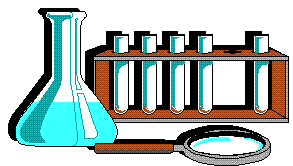
\includegraphics[width=3cm]{../img/science.png}
  &
  \hh{Lexical $+$ Logical Reasoning:} \newline \w{A graduated cylinder would be best to} \newline \w{measure the volume of a liquid} \\
\end{tabular}
\end{frame}
}


\begin{document}
\begin{frame}[noframenumbering]
  \titlepage
\end{frame}

\input motivation.tex


\roadmap{0}
\roadmap{1}


\input naturalli.tex


%%%%%%%%%%%%%%%%%%% 
% Are we done?
%%%%%%%%%%%%%%%%%%% 
\begin{frame}{}
\begin{center}
\hh{Success?} \\
\vspace{2ex}

\includegraphics[height=4cm]{../img/fish.jpg}
\end{center}
\end{frame}

%%%%%%%%%%%%%%%%%%% 
% What are we bad at
%%%%%%%%%%%%%%%%%%% 
\def\title{Not Yet!}
\begin{frame}[noframenumbering]{\title}

\begin{center}
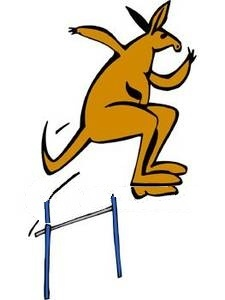
\includegraphics[height=3cm]{../img/hurdle.jpg}
\end{center}

\hh{The Internet doesn't speak in atomic utterances}
\begin{itemize}
\uncover<2->{
  \item Where was Obama born?
    \begin{itemize}
    \item \w{Born in Hawaii, 
             Obama is a graduate of Columbia 
             University and Harvard Law School.} \\
           \uncover<3->{$\Rightarrow$ \w{Obama was born in Hawaii}}.
     \end{itemize}
   \pause
   \pause
   \pause
  \item Let's store the inferred fact instead
}
\end{itemize}
\end{frame}

\roadmap{1}
\roadmap{2}


\input openie.tex


\roadmap{2}
\roadmap{3}


\input science.tex


\input future.tex

\input thanks.tex


%
% References
%
\newcommand{\backupbegin}{
   \newcounter{framenumberappendix}
   \setcounter{framenumberappendix}{\value{framenumber}}
}
\newcommand{\backupend}{
   \addtocounter{framenumberappendix}{-\value{framenumber}}
   \addtocounter{framenumber}{\value{framenumberappendix}} 
}
\backupbegin
\begin{frame}[allowframebreaks]
    \frametitle{References}
    \bibliographystyle{apalike}
    {\small \bibliography{../ref}}
\end{frame}
\backupend

\end{document}
